\documentclass[11pt]{exam}

\usepackage[utf8]{inputenc}
\usepackage{hyperref}
\usepackage[spanish]{babel}
\usepackage{listings}
\usepackage{float}
\usepackage[table,xcdraw]{xcolor}
\usepackage{graphicx}
\usepackage{parcolumns}
\usepackage{array}
\usepackage{caption}

\newenvironment{conditions}
{\par\vspace{\abovedisplayskip}\noindent\begin{tabular}{>{$}l<{$} @{${}\:{}$} l}}
	{\end{tabular}\par\vspace{\belowdisplayskip}}


\definecolor{codegreen}{rgb}{0,0.6,0}
\definecolor{codegray}{rgb}{0.5,0.5,0.5}
\definecolor{codepurple}{rgb}{0.58,0,0.82}
\definecolor{backcolour}{rgb}{0.95,0.95,0.92}

\lstdefinestyle{mystyle}{
	backgroundcolor=\color{backcolour},   
	commentstyle=\color{codegreen},
	keywordstyle=\color{magenta},
	stringstyle=\color{codepurple},
	basicstyle=\ttfamily\footnotesize,
	breakatwhitespace=false,         
	breaklines=true,                 
	captionpos=b,                    
	keepspaces=true,                                   
	showspaces=false,                
	showstringspaces=false,
	showtabs=false,                  
	tabsize=2
}

\lstset{style=mystyle}

\title{Práctica 2}
\author{Laura Rodríguez Navas \\ rodrigueznavas@posgrado.uimp.es}
\date{{\selectlanguage{spanish}\today} }

\pagestyle{plain}

\begin{document}
	
\maketitle

\renewcommand{\tablename}{Tabla}
\renewcommand{\lstlistingname}{Código}

\section{Introducción}\label{introduccion}

Esta práctica se apoya en una plataforma que recrea el videojuego clásico \href{1https://en.wikipedia.org/wiki/Pac-Man}{Pac-Man}. Utiliza una versión muy simplificada del juego para poder desarrollar un sistema de control automático y explorar algunas capacidades del Aprendizaje por Refuerzo aprendidas durante la asignatura. Especialmente, en esta práctica se aplica el algoritmo \textit{Q-learning} para construir un agente Pac-Man que funcione de forma automática, con el objetivo de maximizar la puntuación obtenida en una partida por cada mapa disponible para la práctica: \textit{lab1.lay, lab2.lay y lab3.lay}.  

Asimismo, se presenta este documento donde se describen las tareas de la práctica realizadas, que se dividen en distintas fases (definición de los estados, función de refuerzo, construcción del agente Pac-Man y evaluación), y que se detallan a continuación.

En la sección~\ref{estados} se justifica el conjunto de atributos elegido y su rango para la definición de los estados. Una vez se ha elegido el conjunto de atributos que se van a utilizar para representar cada estado, en la sección~\ref{refuerzo} se detalla el diseño de la función de refuerzo que vamos a emplear y que permitirá al agente Pac-Man lograr su objetivo de maximizar la puntuación obtenida en una partida. Después de esto, en la sección~\ref{codigo} se explica cómo se ha procedido a la construcción del agente con el fin de funcionar bien en todos los laberintos. Cuando se obtiene el agente, en la sección~\ref{resultados} se presentan los resultados de las puntuaciones que ha obtenido en los mapas proporcionados y se añaden comentarios sobre su comportamiento. Finalmente, en la parte final del documento se añaden las conclusiones (sección~\ref{conclusiones}) y un apéndice que contiene métodos auxiliares del código desarrollado en las secciones~\ref{refuerzo} y \ref{codigo}.

\section{Definición de los estados}\label{estados}

En esta sección, a fin de definir los estados, hay que seleccionar unos valores adecuados para los parámetros: \textit{nRowsQTable, alpha, gamma y epsilon}. Primero intentaremos descubrir el valor del parámetro \textit{nRowsQTable}, o que es lo mismo, intentaremos descubrir cuántas filas debe tener la \textit{QTable}. Este valor dependerá de las características seleccionadas para representar los estados, ya que según estas características nos modificará el número de filas de nuestra \textit{QTable}. Nos fijamos en la información que nos proporciona la función \textit{printInfo} durante una ejecución manual del agente, concretamente nos fijamos en la información de los mapas \textit{Walls} y \textit{Food}. Según esta información, que nos indica la presencia y ausencia de paredes y comida en los mapas \textit{Walls} y \textit{Food}, y la información de las direcciones que puede ejecutar el agente Pac-Man: \textit{north, east, south y west}, elegimos 16 características.

\newpage

Las 16 características elegidas son:

\begin{parcolumns}{2}
	\colplacechunks
	\colchunk{
		\begin{itemize}
			\item nearest\_ghost\_north, no\_wall
			\item nearest\_ghost\_south, no\_wall
			\item nearest\_ghost\_east, no\_wall
			\item nearest\_ghost\_west, no\_wall
			\item nearest\_ghost\_north, wall
			\item nearest\_ghost\_south, wall
			\item nearest\_ghost\_east, wall
			\item nearest\_ghost\_west, wall
		\end{itemize}}
	\colchunk{
		\begin{itemize}
			\item nearest\_ghost\_north, no\_food
			\item nearest\_ghost\_south, no\_food
			\item nearest\_ghost\_east, no\_food
			\item nearest\_ghost\_west, no\_food
			\item nearest\_ghost\_north, food
			\item nearest\_ghost\_south, food
			\item nearest\_ghost\_east, food
			\item nearest\_ghost\_west, food
		\end{itemize}}
\end{parcolumns}
\vspace*{3mm}

Según el número de características (16), modificamos el valor del parámetro \textit{nRowsQTable}, de la función \textit{registerInitialState} en la clase \textit{RLAgent} del archivo \textit{bustersAgents.py}, de la siguiente manera:

\begin{lstlisting}[language=python, basicstyle=\footnotesize]
self.nRowsQTable = 16
\end{lstlisting}

También tenemos que modificar los parámetros \textit{alpha, gamma y epsilon}. Pero primero realizamos una pequeña descripción de estos a continuación:

\begin{itemize}
	\item Alpha ($\alpha$). Este valor toma valores entre 0 y 1. Cuando este valor es 0, entonces no hay aprendizaje y siempre se utiliza el valor $Q$ inicial. Cuando este valor es 1, entonces el aprendizaje no conserva ningún porcentaje del valor $Q$. Es decir, si el valor $\alpha$ se acerca a 0, el valor $Q$ no variará mucho, y si el valor $\alpha$ se acerca a 1, el valor $Q$ variará mucho.
	
	\item Gamma ($\gamma$). Este valor toma valores entre 0 y 1. Cuando este valor es 0, entonces el aprendizaje ignorará el valor dado por el modelo de aprendizaje y aprenderá solo con el valor de la recompensa. Cuando este valor es 1, entonces el aprendizaje utilizará el valor total dado por el modelo de aprendizaje.
	
	\item Epsilon ($\epsilon$). Numera los pasos para disminuir el valor $\alpha$. El valor $\alpha$ se reducirá para cada $n$ decisiones tomadas. Por ejemplo, si este valor es 0.01, se reduciría 0.01 el valor de $\alpha$ por cada 10 decisiones tomadas, donde $n$=10.
\end{itemize}

El proceso para elegir los parámetros \textit{nRowsQTable, alpha, gamma y epsilon} se ha realizado con el entrenamiento de una inteligencia simple (sin usar el aprendizaje automático). Esta inteligencia simple se compone de un objetivo muy singular: el agente Pac-Man atacando a uno de los fantasmas en el primer laberinto disponible (\textit{lab1.lay}). Con esa finalidad, ejecutamos el comando \textit{python busters.py -p RLAgent -k 1 -l lab1.lay -n 100} varias veces, con diferentes valores de \textit{alpha, gamma y epsilon} observando el valor resultante \textit{Average Score} de las distintas ejecuciones (ver Figura~\ref{average_score}). El valor \textit{Average Score} nos indicará el valor promedio máximo de las puntuaciones obtenidas durante 100 partidas, o lo que es lo mismo, el valor promedio máximo $Q$ durante 100 partidas. Si este valor es positivo habremos ganado la partida, en caso contrario, habremos perdido la partida.

Por ejemplo, con los valores: \textit{alpha=1} , \textit{gamma=0.8} y \textit{epsilon=0.05} observaremos que el valor \textit{Average Score} será menor que con los valores: \textit{alpha=0.2}, \textit{gamma=0.8} y \textit{epsilon=0.05}. Otro ejemplo, con los valores: \textit{alpha=0.4}, \textit{gamma=0.8} y \textit{epsilon=0.05} observaremos que el valor \textit{Average Score} también será menor que con los valores: \textit{alpha=0.2}, \textit{gamma=0.8} y \textit{epsilon=0.05}. Así, consideramos que la mejor asignación de los parámetros en estos ejemplos son los valores: \textit{alpha=0.2}, \textit{gamma=0.8} y \textit{epsilon=0.05}.

Durante el proceso para elegir los parámetros, los valores de \textit{epsilon} siempre han tomado valores muy próximos a 0, esto refleja un comportamiento aprendido en la \href{https://poliformat.upv.es/portal/site/ESP_0_2835/tool/c07b745a-0cfd-44f0-a7a2-9bb22f80c3f7?panel=Main}{práctica 1} de la asignatura. En esta práctica aprendimos que si en una estrategia $\epsilon$-greedy el valor de $\epsilon$ es más pequeño, entonces la probabilidad de que el agente \textit{Q-learning} tome decisiones aleatorias será menor. Si la aleatoriedad es menor, menor será la inestabilidad del agente \textit{Q-learning}, en este caso la del agente Pac-Man. Como a consecuencia, el promedio del valor máximo $Q$ será mayor, que es equivalente a una mejor puntuación en el videojuego alcanzando el objetivo del agente.
\vspace*{3mm}

Los mejores valores encontrados para los parámetros son los siguientes:
\vspace*{3mm}

\begin{lstlisting}[language=python, basicstyle=\footnotesize]
self.alpha = 0.2
self.gamma = 0.7
self.epsilon = 0.01
\end{lstlisting}

\begin{figure}[H]
	\centering
	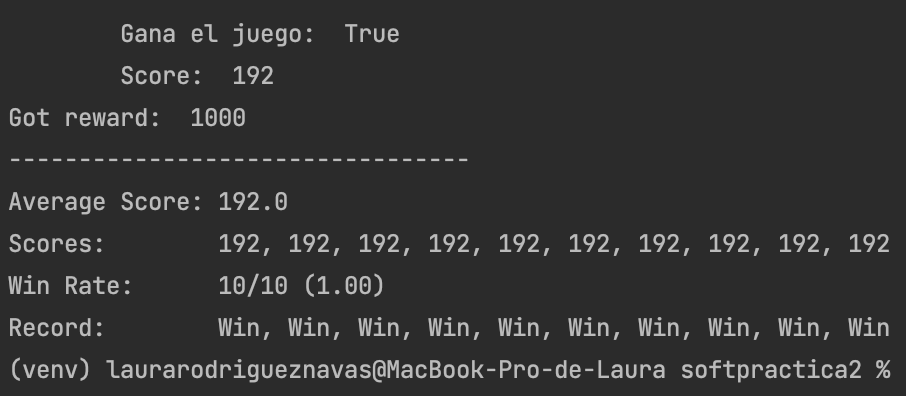
\includegraphics[scale=0.6]{average_score}
	\caption{Ejemplo de ejecución del agente Pac-Man \\ que nos muestra el \textit{Average Score} obtenido.}
	\label{average_score}
\end{figure}


\section{Función de refuerzo}\label{refuerzo}

Una vez que se han adaptado los parámetros del agente Pac-Man ya podemos diseñar la función de refuerzo. La función de refuerzo determinará las recompensas que obtenga el agente. Determinar las recompensas que obtiene el agente con cada acción es clave para su aprendizaje, pues marcará cómo de buenas serán unas acciones frente a otras y por lo tanto determinará qué tipo de comportamientos decidimos potenciar. La siguiente lista enumera las diferentes acciones que he decidido potenciar, con sus valores de recompensa correspondientes:

\begin{itemize}
	\item \textbf{Ganar}: este estado se muestra cuando el agente Pac-Man gana la partida. Ganamos 1000 puntos de recompensa.
	
	\item \textbf{Comer}: este estado se muestra cuando el agente Pac-Man se come a un fantasma. Ganamos 100 puntos de recompensa.
	
	\item \textbf{Lejos de un fantasma y lejos de una pared}: este estado se muestra cuando el agente Pac-Man está al menos a cinco celdas del fantasma más cercano y de la pared más cercana. En este caso, ganamos 1 punto de recompensa.
	
	\item \textbf{Lejos de un fantasma y cerca de una pared}: este estado se muestra cuando el agente Pac-Man está al menos a cinco celdas del fantasma más cercano y está a un máximo de cuatro celdas de la pared más cercana. En este caso, perdemos 1 punto de recompensa.
	
	\item \textbf{Cerca de un fantasma y lejos de una pared}: este estado se muestra cuando el agente Pac-Man está a un máximo de cuatro celdas del fantasma más cercano y está al menos a cinco celdas de la pared más cercana.  En este caso, ganamos 3 puntos de recompensa.
	
	\item \textbf{Cerca de un fantasma y cerca de una pared}: este estado se muestra cuando el agente Pac-Man está a un máximo de cuatro celdas del fantasma más cercano y de la pared más cercana. En este caso, ganamos 2 puntos de recompensa.
	
	\item \textbf{Cerca de una pared}: este estado se muestra cuando el agente Pac-Man está a un máximo de cuatro celdas de la pared más cercana. En este caso, perdemos 3 puntos de recompensa.
	
	\item \textbf{Lejos de una pared}: este estado se muestra cuando el agente Pac-Man está al menos a cinco celdas de la pared más cercana. En este caso, ganamos 1 punto de recompensa.
\end{itemize}

En todas las acciones, el agente Pac-Man recuerda la posición del fantasma más cercano y elige una de las direcciones disponibles: \textit{north, east, south o west} para llegar al fantasma por el camino más corto. Como se puede observar, se han definido las recompensas mediante valores enteros, aunque las acciones dependan de la posición de los fantasmas respecto a la posición del agente. Se ha tomado esta decisión al fin de facilitar el código desarrollado y se han definido los valores de recompensa para cada acción en particular. La elección de los valores concretos de recompensa se han realizado un poco al azar, siguiendo mi propio criterio. La función de refuerzo desarrollada se muestra a continuación:
\vspace*{3mm}

\begin{lstlisting}[caption={Función de refuerzo.}, label={reward}, language=python, basicstyle=\scriptsize]
def getReward(self, state, nextState):
	"""
	Return a reward value based on the information of state and nextState
	"""
	reward = 0
	
	if nextState.isWin():
		return 1000
	
	# distancias al fantasma mas cercano en el siguiente estado
	next_state_ghost_distances = self.getGhostDistances(nextState)
	# distancias al fantasma mas cercano en el estado actual
	actual_state_ghost_distances = self.getGhostDistances(nextState)
	
	# distancia minima al fantasma mas cercano en el siguiente estado
	min_distance_ghost_next_State = min(next_state_ghost_distances, key=lambda t: t[1])[0]
	min_ghost_distance_next_state = nextState.data.ghostDistances[
		min_distance_ghost_next_State]
	# distancia al fantasma mas cercano en el estado actual
	min_distance_ghost_actual_State = min(actual_state_ghost_distances, key=lambda t: t[1])[0]
	min_ghost_distances_actual_state = state.data.ghostDistances[min_distance_ghost_actual_State]
	
	# numero de fantasmas en el estado actual
	number_ghost_actual_state = len(list(filter(lambda d: d is not None, 
		state.data.ghostDistances)))
	# numero de fantasmas en el siguiente estado
	number_ghost_next_state = len(list(filter(lambda d: d is not None, 
		nextState.data.ghostDistances)))
	
	# distancia a la pared mas cercana en el estado actual
	actual_state_has_walls = self.directionIsBlocked(state,
	state.getGhostPositions()[min_distance_ghost_next_State])
	# distancia a la pared mas cercana en el siguiente estado
	next_state_has_walls = self.directionIsBlocked(nextState,
	nextState.getGhostPositions()[min_distance_ghost_next_State])
	
	# come fantasma
	if number_ghost_next_state < number_ghost_actual_state:
		reward += 100
	
	# mas lejos de un fantasma y lejos de una pared, no come
	if min_ghost_distance_next_state < min_ghost_distances_actual_state \
			and not actual_state_has_walls \
				and number_ghost_next_state == number_ghost_actual_state:
		reward += 1
	
	# mas lejos de un fantasma y cerca de una pared, no come
	elif min_ghost_distance_next_state < min_ghost_distances_actual_state \
			and actual_state_has_walls \
				and number_ghost_next_state == number_ghost_actual_state:
		reward -= 1
	
	# mas cerca de un fantasma y lejos de una pared, no come
	elif min_ghost_distance_next_state > min_ghost_distances_actual_state \
			and not actual_state_has_walls \
				and number_ghost_next_state == number_ghost_actual_state:
		reward += 3
	
	# mas cerca de un fantasma y cerca de una pared, no come
	elif min_ghost_distance_next_state > min_ghost_distances_actual_state \
		and actual_state_has_walls \
			and number_ghost_next_state == number_ghost_actual_state:
		reward += 2
	
	# cerca de una pared, no come
	if not actual_state_has_walls and next_state_has_walls \
			and number_ghost_next_state == number_ghost_actual_state:
		reward -= 3
		
	# lejos de una pared, no come
	elif actual_state_has_walls and not next_state_has_walls \
			and number_ghost_next_state == number_ghost_actual_state:
		reward += 1
	
	return reward
\end{lstlisting}

Los métodos auxiliares de la función de refuerzo como el método \textit{getGhostDistances}, que muestra las distancias entre los fantasmas y el agente Pac-Man (ver Código~\ref{getGhostDistances}), y el método \textit{directionIsBlocked}, que nos indica si la dirección tomada por el agente se bloquea por una pared (ver Código~\ref{directionIsBlocked}), se incluyen en la sección~\ref*{apendice_reward}.

\section{Código desarrollado}\label{codigo}

Una vez que hemos seleccionado los parámetros que vamos a utilizar para representar cada estado, y hemos desarrollado la función de refuerzo que vamos a emplear (ver Código~\ref{reward}), procedemos a la construcción del agente Pac-Man. La implementación del agente consiste en ir determinando el estado actual en que se encuentra. Dado este estado, se elige la acción de acuerdo con los valores $Q$. Una vez elegida la acción, se determina cuál es la dirección más apropiada para la acción dada. A la hora de elegir la siguiente acción, se actualiza el valor $Q$ para el estado y la acción anterior, dado el estado actual obtenido y la mejor acción que devuelve la fórmula expresada en la ecuación~\ref{formula}, que podemos observar en la página siguiente. Finalmente dado el estado actual, el proceso comenzará de nuevo eligiendo la siguiente acción. Este procedimiento se recoge en la función \textit{update} (ver Código~\ref{update}), que lleva a cabo el algoritmo \textit{Q-learning}. 

Como se ha visto ya en la \href{https://poliformat.upv.es/portal/site/ESP_0_2835/tool/c07b745a-0cfd-44f0-a7a2-9bb22f80c3f7?panel=Main}{práctica 1} de la asignatura, los valores de la tabla $Q$ únicamente son actualizados cuando se cambia de estado, es decir, si al tomar una acción, el agente se mantiene en el mismo estado, la tabla $Q$ no se actualiza, sino que la recompensa se acumula, de forma que se suman todas las recompensas obtenidas mientras se permanece en un estado, y es cuando se pasa al siguiente, el momento de modificar la tabla $Q$. 

\newpage

La fórmula para obtener el nuevo valor $Q$:

\begin{equation}\label{formula}
	Q_{(t+1)}(s_{t},a_{t}) = (1-\alpha) * Q_{t}(s_{t},a_{t}) + \alpha * (R(s_{t},a_{t})) + V_{t}(s_{t+1}) - Q_{t}(s_{t},a_{t})
\end{equation}

donde,

\begin{conditions}
	Q_{(t+1)}(s_{t},a_{t}) & es el nuevo valor $Q$ dado el estado anterior $s_{t}$ y la acción anterior $a_{t}$. \\
	\alpha & es la tasa de aprendizaje. \\
	R(s_{t},a_{t}) & es el valor de recompensa dado el estado anterior $s_{t}$ y la acción anterior $a_{t}$.	\\
	Q_{t}(s_{t},a_{t}) & es el antiguo valor de $Q$ dado el estado anterior $s_{t}$ y la acción anterior $a_{t}$.	\\
	V_{t}(s_{t+1}) & es el valor de aprendizaje dado el nuevo estado $s_{t+1}$.
\end{conditions}

La función \textit{update} que lleva a cabo el algoritmo \textit{Q-learning}:
\vspace*{3mm}

\begin{lstlisting}[caption={Función update.}, label={update}, language=python, basicstyle=\footnotesize]
def update(self, state, action, nextState, reward):
	"""
	The parent class calls this to observe a
	state = action => nextState and reward transition.
	You should do your Q-Value update here
	"""
	reward = reward + self.getReward(state, nextState)  # actualizar recompensa
	
	print "Started in state:"
	self.printInfo(state)
	print "Took action: ", action
	print "Ended in state:"
	self.printInfo(nextState)
	print "Got reward: ", reward
	print "---------------------------------"

	# buscar el estado actual en la memoria de estados
	state_position = self.computePosition(state)
	action_position = self.actions[action]  # elegir accion
	# actualizar la tabla Q con la accion elegida
	self.q_table[state_position][action_position] = (1 - self.alpha) * 
		self.q_table[state_position][action_position] + self.alpha * (reward + 
			self.gamma * self.getValue(nextState))

	if nextState.isWin():
	# If a terminal state is reached
		self.writeQtable()
\end{lstlisting}

En la función \textit{update}, primero actualizamos el valor de la recompensa. Esto se debe a que en la función \textit{getReward} (ver Código \ref{reward}), el valor de la variable \textit{reward} inicialmente siempre es 0. Después buscamos el estado actual en la memoria de estados con la función \textit{computePosition} (ver Código~\ref{computePosition}), método que se incluye en la sección~\ref{apendice_update}. El agente Pac-Man aprende modificando los valores $Q$ (valores que hay almacenados en la tabla $Q$), de forma que cuando se realiza la acción \textit{action\_position} desde el estado \textit{state\_position}, es el valor $Q(s,a)$ el que se ve modificado de acuerdo a la fórmula expresada en la ecuación~\ref{formula}. Con la finalidad de que el agente pueda aprender, necesita tener a mano todos los estados que ya haya visitado anteriormente, para poder detectar en cuál de ellos se encuentra a medida que va jugando y, en caso de encontrarse en una situación nueva, registrarla para utilizarla posteriormente. En la implementación de la función \textit{statesMemory}, método que se incluye en la sección~\ref{apendice_update}, estos estados se guardan en forma de lista a medida que se van descubriendo (ver Código~\ref{statesMemory}).
\vspace*{3mm}

Una vez modificado el agente, observamos su comportamiento en uno de los laberintos disponibles de la práctica, ejecutándolo con el siguiente comando:

\begin{lstlisting}[language=python, basicstyle=\footnotesize]
python busters.py -p RLAgent -k 1 -l lab1.lay -n 100
\end{lstlisting}

Con ello, hemos ejecutado durante 100 partidas el agente que acabamos de crear en el laberinto \textit{lab1}, que únicamente tiene un fantasma (ver Figura). Lo volvemos a ejecutar, pero esta vez en el laberinto \textit{lab2} que tiene dos fantasmas, con el uso del siguiente comando:

\begin{lstlisting}[language=python, basicstyle=\footnotesize]
python busters.py -p RLAgent -k 2 -l lab2.lay -n 100
\end{lstlisting}

Finalmente, también lo ejecutamos en el último de los laberintos disponibles de la práctica, el laberinto \textit{lab3}, que tiene 3 fantasmas, pared en el interior del laberinto y un punto.

\begin{lstlisting}[language=python, basicstyle=\footnotesize]
python busters.py -p RLAgent -k 3 -l lab3.lay -n 100
\end{lstlisting}

El agente Pac-Man toma decisiones cada vez que llega a una intersección, momento en que mira el estado del juego, ve en qué situación se encuentra, y en base a los conocimientos aprendidos toma la decisión de moverse en una dirección u otra. También, en aquellos momentos en que se le proporciona información acerca de los fantasmas, el agente también toma decisiones en el momento en que percibe a un fantasma demasiado cerca de él, momento en el cual decide atacar, aunque no se encuentre en una intersección. El agente aprende a perseguir a los fantasmas, que son los que le reportan mayor beneficio. Elige caminos que contienen la mayor cantidad de fantasmas, desviándose a veces si ve que tiene un fantasma comestible cerca.

\section{Resultados}\label{resultados}

En esta sección exponemos los resultados obtenidos en las ejecuciones realizadas en la sección anterior (ver sección~\ref{codigo}), además sacamos algunas conclusiones con respecto a los resultados. Los resultados obtenidos son:

\begin{table}[H]
	\centering
	\begin{tabular}{|c|c|} 
		\hline
		Mapa & Average Score \\ 
		\hline
		1 & 191.89 \\ 
		2 & 390.96 \\
		3 & 578 \\
		\hline
	\end{tabular}
	\caption{Resultados de las ejecuciones del agente Pac-Man.}
	\label{resultados_ejecuciones}
\end{table}

Podemos ver que la técnica de \textit{Q-learning} implementada en el agente Pac-man es lo suficientemente inteligente para vencer en los tres mapas.
 
\section{Conclusiones}\label{conclusiones}

\textit{Q-learning} en estos casos, es sin duda un método que parece efectivo. Sin embargo, requiere realizar muchos experimentos para estudiar la viabilidad de las soluciones propuestas. En concreto lo que más problemas me ha dado ha sido la tarea de diseñar los casos, y de cómo utilizar la información que contienen para hacer que el sistema evolucione a medida que se simulan las partidas. Conseguir un equilibrio para que los casos no sean demasiado específicos (y por tanto se reutilicen pocas veces), ni tampoco demasiado generales (y no aporten soluciones especialmente útiles), es complicado y requiere de muchas pruebas hasta encontrar los parámetros que mejor se adaptasen al objetivo perseguido.

Personalmente uno de los mayores retos de esta práctica ha sido la implementación de todo el código para operar con el agente Pac-Man. El videojuego que se utiliza parece a priori sencillo, pero representa un dominio que se puede volver extremadamente complejo cuando pretendes que un agente aprenda a jugar. Un jugador humano procesa información visual y la aplica muy rápido cuando toma decisiones, pero para conseguir que una máquina haga lo mismo, se necesita un grado de abstracción de esa información que en ocasiones se ha vuelto muy difícil de conseguir. Ha sido de gran ayuda que muchas personas hayan resuelto este problema de diferentes maneras, ya me ha dado la posibilidad de aprender y tener una implementación base con la que guiarme.

Todo el contenido de esta práctica se puede encontrar en el repositorio personal de GitHub: \url{https://github.com/lrodrin/masterAI/tree/master/A21/softpractica2}.

\section{Apéndice}\label{apendice}

\subsection{Métodos de la función \textit{get\_reward}}\label{apendice_reward}

\begin{lstlisting}[caption={Función getGhostDistances.}, label={getGhostDistances}, language=python, basicstyle=\footnotesize]
def getGhostDistances(gameState):
	"""
	Return distances to each of the ghosts on the map.
	"""
	return [(i, distance) for i, (distance, alive) in enumerate(zip(
		gameState.data.ghostDistances, gameState.getLivingGhosts()[1:])) if alive]
\end{lstlisting}

\begin{lstlisting}[caption={Función directionIsBlocked.}, label={directionIsBlocked}, language=python, basicstyle=\footnotesize]
def directionIsBlocked(gameState, ghost_position):
	"""
	Return True if directions are blocked (walls) and False otherwise (no walls).
	It also returns distances to blocking elements and non-blocking elements.
	"""
	walls = gameState.getWalls()
	walls_array = np.array(walls.data)
	pacman_position = gameState.getPacmanPosition()
	
	x_min = min(pacman_position[0], ghost_position[0])
	x_max = max(pacman_position[0], ghost_position[0]) + 1
	y_min = min(pacman_position[1], ghost_position[1])
	y_max = max(pacman_position[1], ghost_position[1]) + 1
	if y_min < 3:
		y_min = 3
	
	grid_beetween = walls_array[x_min:x_max, y_min:y_max]
	if len(grid_beetween) == 0:
		return False
	
	return np.any(np.all(grid_beetween, axis=1)) or np.any(np.all(grid_beetween, axis=0))
\end{lstlisting}

\subsection{Métodos de la función \textit{update}}\label{apendice_update}

\begin{lstlisting}[caption={Función computePosition.}, label={computePosition}, language=python, basicstyle=\footnotesize]
def computePosition(self, state):
	"""
	Compute the row of the qtable for a given state.
	"""
	pacman_ghost_direction, ghost_position = self.statesMemory(state)
	hasWall = self.directionIsBlocked(state, ghost_position)
	actions_value = 0
	for i, direction in enumerate(pacman_ghost_direction):
		actions_value += min(self.actions[direction], 2) + i * 4
	return int(hasWall) * 8 + actions_value
\end{lstlisting}

\begin{lstlisting}[caption={Función statesMemory.}, label={statesMemory}, language=python, basicstyle=\footnotesize]
def statesMemory(self, gameState):
	"""
	Create states memory.
	"""
	# posicion de pacman
	pacman_position = gameState.getPacmanPosition()
	
	# distancia minima al fantasma mas cercano
	living_ghosts_distances = self.getGhostDistances(gameState)
	min_distance_ghost_index = min(living_ghosts_distances, key=lambda t: t[1])[0]
	
	# posicion del fantasma mas cercano
	nearest_ghost_position = gameState.getGhostPositions()[min_distance_ghost_index]
	
	pacman_ghost_direction = []
	
	if (pacman_position[1] - nearest_ghost_position[1]) != 0 \
			and (pacman_position[1] - nearest_ghost_position[1]) > 0:
		pacman_ghost_direction.append("South")
	if (pacman_position[1] - nearest_ghost_position[1]) != 0 \
			and (pacman_position[1] - nearest_ghost_position[1]) < 0:
		pacman_ghost_direction.append("North")
	if (pacman_position[0] - nearest_ghost_position[0]) != 0 \
			and (pacman_position[0] - nearest_ghost_position[0]) > 0:
		pacman_ghost_direction.append("West")
	if (pacman_position[0] - nearest_ghost_position[0]) != 0 \
			and (pacman_position[0] - nearest_ghost_position[0]) < 0:
		pacman_ghost_direction.append("East")
	
	return pacman_ghost_direction, nearest_ghost_position
\end{lstlisting}

\end{document}
